\documentclass[10pt,a4paper]{article}
\usepackage[margin=1.6cm]{geometry}
\usepackage[T1]{fontenc}
\usepackage{lmodern}
\usepackage{amsmath}
\usepackage{booktabs}
\usepackage{enumitem}
\usepackage{xcolor}
\usepackage{graphicx}
\usepackage[font=small,labelfont=bf]{caption}
\graphicspath{{../results/}}
\definecolor{ocean}{RGB}{20,70,110}
\setlist{nosep,leftmargin=1.2em}
\setlength{\parskip}{3pt}\setlength{\parindent}{0pt}
\newcommand{\head}[1]{\par\vspace{4pt}{\bfseries\color{ocean}#1}\par\vspace{1pt}}

\begin{document}
{\large\bfseries\color{ocean} Memo: progress and decisions, paper from the EEE4022S thesis}\\[1pt]
{\small To: Robyn Verrinder \quad From: Amir Dollie \quad Meeting: Thu 26 Nov 2026, 12h30 \quad (moved forward from Fri 27 Nov)}

\head{1. Forward-model convergence (plan item F1): resolved}
The thesis reported that the EMM did not converge ($[M,20,20]$ never met $d<0.1$). It does converge. The solver is correct: energy is conserved to $10^{-15}$, symmetry holds, and every change reproduces the old results to machine precision. The apparent non-convergence was three independent truncation errors measured together (Figures~\ref{fig:floor} and~\ref{fig:towers}).
\begin{itemize}
\item \textbf{Open-water vertical modes ($M_o$):} a slow beat with a period of $1/\gamma\approx690$ modes, which made every step of the thesis ladder stall (Fig.~\ref{fig:floor}). This tower is mathematically cheap, so it can now be taken to $M_o=20\,000$--$40\,000$ (Fig.~\ref{fig:towers}a).
\item \textbf{Plate vertical modes ($M$):} a clean power law, error $\sim M^{-1.7}$, from the edge-corner singularity (Fig.~\ref{fig:towers}b).
\item \textbf{Angular orders ($N$):} $N=10$ is fine for the reference floe but leaves a \textbf{2\% error} for floes of twice the radius. $N$ is a resolution setting, not a floe property. It is fixed conservatively from the \emph{largest} radius in the search range ($N=25$ covers $2R_0$ plus a 30\% margin). Extra orders cost only time and cannot bias the result.
\end{itemize}
Against a converged (extrapolated) reference, in the inverse's own Fisher units (target $d\le0.1$):

\begin{center}\small
\begin{tabular}{@{}lcccc@{}}
\toprule
Truncation & p0 & $R=2R_0$ & $(\beta_0/2,2R_0)$ & $(2\beta_0,2R_0)$ \\
\midrule
Thesis $[50,10,10]$ & 8.8 \;(0.29\% in $\beta$) & 23.4 & 27.1 & 8.5 \\
$[400,10,N^*,2{\times}10^4]$ & 0.26 & 0.21 & 0.26 & 0.13 \\
$[800,10,N^*,2{\times}10^4]$ & \textbf{0.087} \;(0.004\%) & \textbf{0.062} & \textbf{0.084} & \textbf{0.038} \\
\bottomrule
\end{tabular}
\end{center}
\textbf{Conclusions.}
\begin{itemize}
\item The thesis model was far from converged \emph{statistically} but not \emph{physically}: at most 0.29\% in $\beta$.
\item The large-floe A1 classes survive with the converged model. They are set by the Welch bias, so the thesis conclusion about the upper identifiability boundary stands.
\item The V1a truncation numbers must be redone: the thesis compared against an unconverged truth, which also differed in $N$.
\item The code is fixed, tested and pushed. It includes overflow-safe Bessel functions, root finding 550$\times$ faster, and the split-truncation solver.
\end{itemize}
Remaining confirmations, not open problems: spot-checks at a soft or small floe and a MIZ floe; a reciprocity check; reproducing a published Montiel PVC curve.

\head{2. Questions}
\begin{enumerate}
\item \textbf{Production model.} Adopt $[800,10,25,20000]$ for all studies ($N^*$ in the table is the minimum each floe needs): within target everywhere, $\sim$8\,min per scenario, with the A1 sweep run overnight. The alternative is $[400,\ldots]$ at a third of the cost, with $d\approx0.13$--$0.28$ carried in the error budget.
\item \textbf{Identifiability classes (F10).} The thesis class is decided almost entirely by $d_{\rm tot}\le0.5$. That tests whether the error bars are honest, not whether the estimate is accurate. Because $\sigma_{\ln\beta}\approx0.05\%$, it fails on physically negligible errors: the p0 class flips between Identifiable and Marginal on a 0.008\% change in $\beta$, and quieter sensors or longer records make it \emph{worse}.\\
\emph{Proposal:}
\begin{itemize}
\item an \emph{accuracy class} on the total error $e_\beta=\sqrt{\sigma^2+\text{bias}^2}$, for example Identifiable $\le5\%$ and Marginal $\le20\%$;
\item $d_{\rm tot}\le0.5$ kept as a \emph{calibration flag}, with bias-aware intervals quoted where it fails;
\item old and new rules shown side by side, with a tolerance ladder (1/5/10/20\%), because the thesis classes were pre-registered.
\end{itemize}
Do you agree with the split, and with the tolerances?
\item \textbf{New robustness study (F4).} Sensor timing offset \emph{and clock drift} (independent $\pm20$\,ppm clocks can drift about 0.26\,s apart over 109\,min), plus relative gain and tilt errors. The outcome is a synchronisation specification for the basin rig. Is this in scope as the main new study?
\item \textbf{Venue and framing.} \emph{Wave Motion} as the primary target, with a basin-scale title (not ``Antarctic'') and the field link as a scaling argument. Agreed?
\item \textbf{Length of paper.} What length and format should the draft target?
\end{enumerate}

\head{3. Next steps if agreed}
Adopt the truncation and rerun the paper's studies (Fri to Mon), reclassify under the agreed rules, then: the complete Welch-bias model (F2), operational-covariance checks (F3), the timing study (F4), and the results freeze on Fri 4 Dec. Draft to you and Malcolm on Wed 9 Dec.

\clearpage
\head{Supporting figures}
All errors are relative changes in the three transmissibilities $T$ (sensors s2, s6, s14 against s26) at the reference floe p0, the quantity the inverse actually sees.

\begin{figure}[h]
\centering
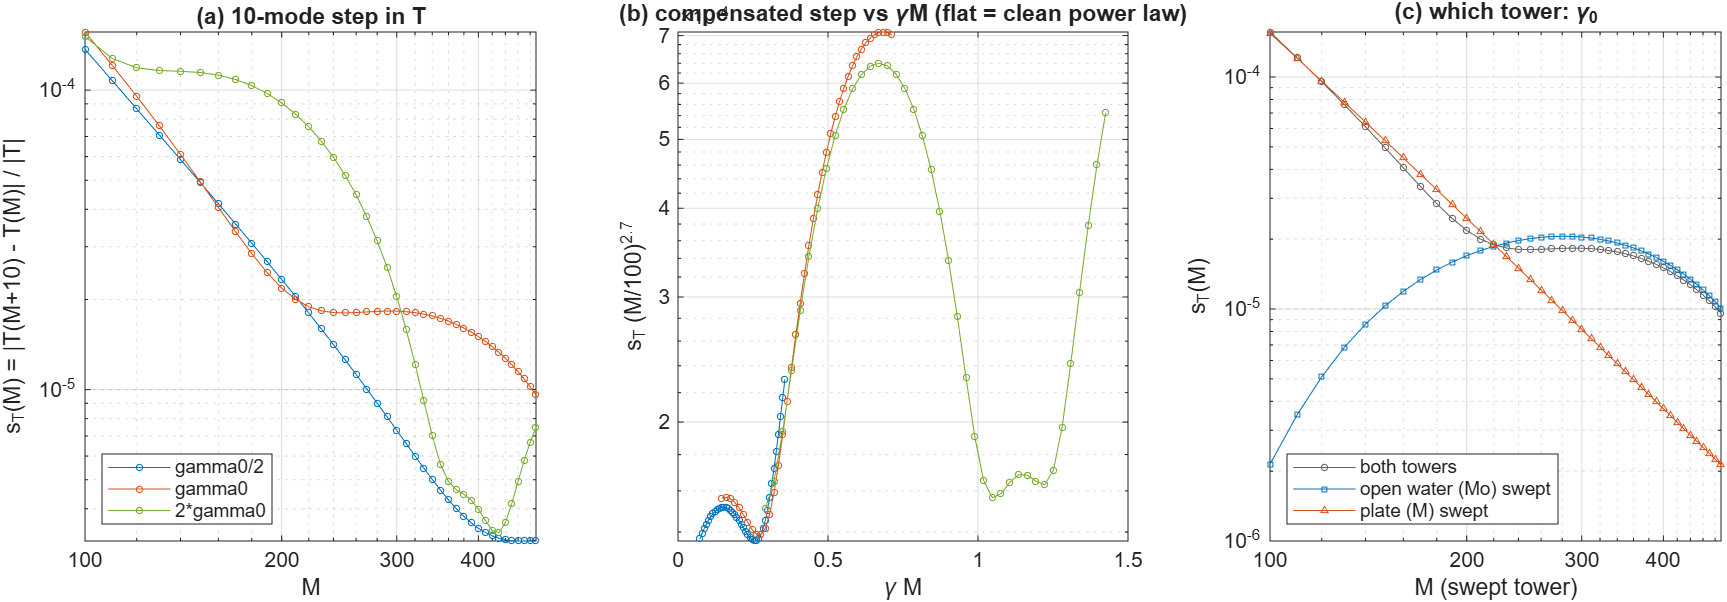
\includegraphics[width=\linewidth]{diag_F1_floor.png}
\caption{\textbf{Why the thesis ladder stalled} (8.5\,rad/s; both mode sets truncated together, $M_o=M$, as in the thesis).
(a) Change in $T$ when 10 modes are added. For the real floe ($\gamma_0$) it goes flat between $M\approx220$ and 330: the ``floor''. The flat stretch moves with the draught (earlier at $2\gamma_0$, later at $\gamma_0/2$), which a bug or rounding error would not do.
(b) The same data with the expected $M^{-2.7}$ decay removed, plotted against $\gamma M$. A clean power law would be flat. Instead, all three draughts collapse onto one slow oscillation with a period of about 1 in $\gamma M$, i.e.\ $1/\gamma\approx690$ modes: a beat between the open-water modes, which span the full depth, and the edge basis, which spans only the depth below the plate.
(c) The two mode sets truncated separately at $\gamma_0$. The plate modes alone (orange) converge as a clean power law ($p\approx1.74$). The open-water modes alone (blue) carry the whole stall. With both tied together (grey), the open-water beat hides the plate's progress from $M\approx220$ upwards.}
\label{fig:floor}
\end{figure}

\begin{figure}[h]
\centering
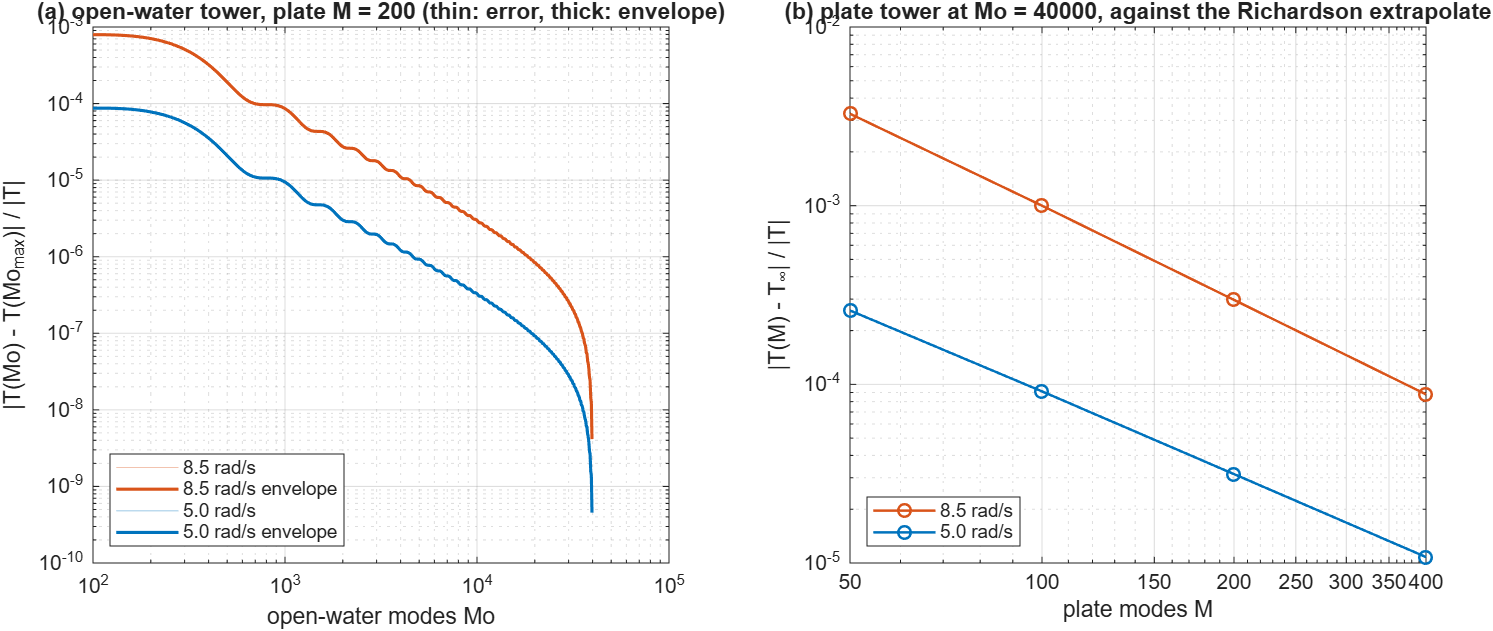
\includegraphics[width=\linewidth]{diag_F1_Mo_ladder.png}
\caption{\textbf{Once separated, both mode sets converge.}
(a) Open-water modes from $M_o=100$ to 40\,000 (plate fixed at $M=200$), at 8.5 and 5.0\,rad/s. The error (thin) equals its envelope over one beat period (thick), so it falls as a staircase and never rises again. It reaches about $4\times10^{-7}$ at $M_o=40\,000$, and taking $M_o$ that far costs only seconds. The plunge at the right edge is an artefact: the error is measured against $M_o=40\,000$ itself.
(b) Plate modes from $M=50$ to 400 (open water at $M_o=40\,000$) against the Richardson extrapolate. Straight lines on log--log axes: a clean power law, $p\approx1.76$ at 8.5\,rad/s and $1.54$ at 5.0\,rad/s, falling from $3\times10^{-3}$ at the thesis's $M=50$ to under $10^{-4}$ at $M=400$. Later runs to $M=800$ and 1600 confirmed the rate is stable. Together, the two panels give the production choice: large $M_o$ (nearly free) and $M=800$ (the G1 table).}
\label{fig:towers}
\end{figure}

\end{document}
